\documentclass[10pt,conference]{IEEEtran}
\usepackage[cmex10]{amsmath}
\usepackage{hyperref}
\usepackage{graphicx}
\usepackage{bbm}
\usepackage{wasysym}
\hyphenation{op-tical net-works semi-conduc-tor}

\begin{document}
\title{Non-Parametric Genomic Fourier Power Spectra Filter Designs }

\author{Micah Thornton\\
Lyda Hill Department of Bioinformatics\\
University of Texas Southwestern\\
\href{mailto:micah.thornton@utsouthwestern.edu}{micah.thornton@utsouthwestern.edu}
\and 
Monnie McGee\\
Department of Statistical Science\\
Southern Methodist University\\
\href{mailto:mmcgee@smu.edu}{mmcgee@smu.edu}}

\IEEEtitleabstractindextext{%
\begin{abstract}
The comparison of genomic sequences is a important undertaking, for example in phylogenetic and differential sequence analyses. In this work we describe three filter designs that 
can be applied to genomic power spectra (PS) of any lengths to reduce their size while maintaining the relative  
distances which they provide and are relevant for data reduction, sorting, and correlation studies of an ensemble of sequences. Specifically we present: \textit{Minimal Variance Filtering} (MVF), where the 
subsets of coefficients with the highest variance across a sample are selected, \textit{Automated Filter 
Learning} (AFL), where a set of linear combinational filters are learned automatically by a 1-D deep convolutional neural network attempting to classify sequences on region of origin, and \textit{Maximal Variance Principal Components Filters} (MVPCF) that provide a set of filters in the Principal component loadings determined among the highest variance elements of the PS for a sample.  We provide a comparison of these approaches by examining their conservation of distances produced by 
the entire PS, and conclude with remarks about the benefits and drawbacks of each method while providing future avenues of pursuit for this research. 
\end{abstract}
\begin{IEEEkeywords}
genomic signal analysis,  genomic power spectra filtering,  genetic sequence analysis, genomic power spectra convolutional neural networks, biomolecular sequence frequency filtering, Virus genomic Fourier power spectra filtering. 
\end{IEEEkeywords}}

\maketitle

\IEEEdisplaynontitleabstractindextext

\IEEEpeerreviewmaketitle

\vspace{-0.5 em}
\section{Introduction \footnote{A video may be viewed here: \href{https://youtu.be/9nqm2Mn7LVU}{https://youtu.be/9nqm2Mn7LVU}}}
\label{sec:int}

\noindent Genomic sequences  contain the essential information required to instantiate and replicate organisms or non-living matter such as viruses and proteins.
They can be considered radix-four signals as they consist of repetitive series of four base nucleotides (NTs): 
adenine, cytosine, guanine, and thymine, in DNA where thymine is replaced by uracil in transcribed  RNAs  \cite{Ana01}. 
The analogy to a radix-four signal does not lend itself to further biological 
attributes such as epigenetic signals.  \cite{Shu17} \cite{San19}.
The NT sequences alone have been used in a recent application of  information and fluctuation theory to genomic signals
\cite{Dem14}.  
In this work, we build on the application of spectral analysis to genomic signals utilizing a version of the mixed radix Fourier PS\cite{Sin69}.
We consider the utility of filtered subsets of PS coefficients produced by a few techniques, with special focus on preserving relative distances 
captured by the entire un-filtered genomic PS. 
To this end, we apply our non-parametric data-driven filters to a subset of SARS-CoV-2 virus genomes curated by the GISAID \cite{gisaid} 
Initiative. 

This remainder of this paper is arranged thusly: first, critical prior works are discussed through a description of the signal flow for 
genomic information from genetic material to the PS in Section \ref{sec:pw}.  Second, the three novel PS filter designs are described in detail in Section \ref{sec:meth}. Following this, a case study of application for the three filters in a sampling of SARS-CoV-2 
virus genomes, curated by the GISAID Initiative and downloaded on August 20, 2020, is demonstrated.  In Section \ref{sec:res}. In concluding section \ref{sec:conc}, comparisons of the approaches are discussed and remarks are made on the benefits and drawbacks of the three filter designs. Also, an 
assessment of the filtered PS in the case study is given and extensions to the work are provided.  
A discussion of software complete with video demonstration link follow the conclusion.

\vspace{-0.5 em}
\section{Prior Works}
\label{sec:pw}
\noindent The application of Discrete-Time Fourier Transforms (DFT) to genomic signals, with``time'' referring to loci, dates back to the early 1990`s.  
Anastassiou provides a summary of these and other genomic signal processing techniques \cite{Ana01}.
Yin et al. suggested the use of the genomic PS as numerical summaries for distance calculations and phylogeny construction
\cite{yin20, yin14, yin15,pei19,Hoa15}.
To render sequences of different lengths comparable, the genomic PS are subject to an even stretching (scaling) procedure defined in Yin et al.'s 2014 work, 
where shorter PS are extended so all genomic sequences are represented by PS of the same lengths. 

\subsection{Encoding \& Transforming Genomic Sequences}
\noindent Genomic/proteomic signals when digitized can be stored in ASCII encoded files in FASTA/Q format.  
FASTA stands for Fast-All  \cite{Lip85}, in reference to the storage capabilities of the format for any alphabet based sequence.
For biomolecular sequences these are mostly genetic or proteomic sequences.  
NT sequences are presented in the organic materials such as DNAs and RNAs, enormously dense and ultra resilient storage systems of natural origin. 
The harvested organic material having been analyzed by sequencing technology \cite{Met10} \cite{Sla18} yields a NT sequence, stored either directly in FASTA/Q or other formats,such as intensity images for micro-array data. 

Sequenced genomic data is processed using bioinformatic procedures towards a certain aim. 
If assembly or alignment is researcher's goal a sequence assembler or aligner may be used.  
An assembler is a tool that builds a long sequence from fragmented shorter sequences such as those produced during sequencing.
An aligner uses a reference sequence (sometimes built previously using an assembler) and places shorter sequences (called reads)
 along the reference.
Popular aligners for regular DNA sequencing include: HISAT, \cite{kim15} HISAT2\cite{Kim19}, bowtie2 \cite{lan12}, and BWA \cite{li09}.
Some special purpose aligners for handling sequencing data from NT-conversion, such as HISAT3N \cite{Zha20} have also been developed.

Following alignment or assembly, sequences are stored in FASTA/Q after intermediate processing through other more convenient formats such as SAM/BAM/CRAM. 
If a researcher working with the sequences is going to generate the PS for this genomic sequence in efforts to compare it to other sequences of the same kind they must first determine whether they wish it to be encoded using four-vectors or two-vectors \cite{Vos92}.
This decision does not always result in contesting relative distance calculations further down the line, but it was suggested by Yin et al in 2015 \cite{yin15} 
that encoding using two-vectors with a strategy picked to attempt to ``balance'' the signals will provide better PS representations.  
The mapping into four-vectors is Equation \ref{eqn:fvec}, and one possible two-vector encoding, for reference, is Equation \ref{eqn:tvec}. 

\noindent 
\begin{align}
\begin{split}
\label{eqn:fvec}
V_4[\cdot] &\equiv \{A,C,G,T/U\} \mapsto \\
& \{ [1,0,0,0]^T,[0,1,0,0]^T,[0,0,1,0]^T,[0,0,0,1]^T\}
\end{split}
\end{align}


\noindent 
\begin{align}
\begin{split}
\hspace{-8 em}
\label{eqn:tvec}
V_{2AT}[\cdot] &\equiv\{A,C,G,T/U\} \mapsto \\
& \{ [0,-1]^T,[-1,0]^T,[1,0]^T,[0,1]^T\}
\end{split}
\end{align}


The PS, as described by Singleton in 1969 \cite{Sin69}, is computed for each row of the encoded genomic signals (four times for $V_4$, and two for $V_{2AT}$).
The resulting PS are then averaged together by position, providing a single PS of the same length as the initial signal. 
If this PS is to be compared to others in an ensemble of signals, a direct comparison method is the 
computation of the Euclidean distance between the PS. 

However, it is often that there are insertions and deletions in two genomic sequences of the same kind 
which render their PS incomparable directly due to the length disparity. 
When this is the case, the researcher may compensate by applying a procedure that stretches the 
shorter sequence to align it's length with that of the longer sequence. 
Such a procedure \cite{yin15} is described in detail in the next section. 


\subsection{Evenly Scaling Power Spectra} 
\noindent  The procedure scans through the shorter sequence taking either a single PS coefficient, or a pair of coefficients, and 
averages them to produce a signal of the same length as that of the longer.  
The formula used is expressed in Equation \ref{eq:evscal}. 

Formally, let $A_n$ denote the original power spectrum of length $n$, and $A_m$ denote the extended power spectrum of length $m$, where $m > n$ and $k=1,2,\dots,m$ indexes the scaled signal. The even scaling operation from $A_n$ to $A_m$ is given by

\begin{align}
\begin{split}
&A_m(k)=\\
&\begin{cases} A_n(Q) & \mbox{if } Q\in Z^+\\
 A_n(R) + (Q-R)(A_n(R+1)-A_n(R)) & \mbox{if } Q  \notin Z^+
\end{cases}
\label{eq:evscal}
\end{split}
\end{align}


\noindent where $Q = \frac{kn}{m}$ and $R = \lfloor \frac{kn}{m} \rfloor$ \cite{yin15}. The \textit{even scaling procedure} is extensible to signal length differences of up to one half the size of the smaller signal without providing substantive loss in terms of information content, although systematically it may be applied in cases where the length difference exceeds this boundary.

\vspace{-1 em}
\begin{figure}[h!]
\caption{Genomic Signal Flow Diagram for Mixed-Radix Power Spectra Calculation} 
\label{fig:fftflow} 
\begin{center} 
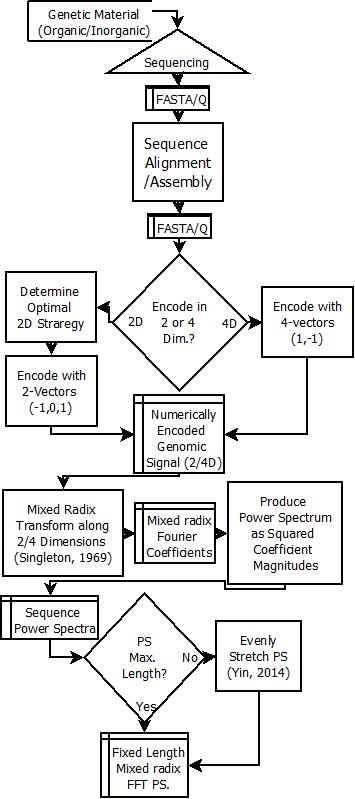
\includegraphics[scale=0.6]{Images/Files/GenomicFFTSignalFlow.png}
\end{center} 
\end{figure} 
\vspace{-1 em} 

A signal flow diagram describing the information stream from the genetic material to the produced \textit{evenly scaled} PS is represented in Figure \ref{fig:fftflow}.  
The \textit{evenly scaled} PS are the numerical summaries of the sequences to which 
the novel filtering procedures are applied.
These three filtering approaches are introduced in the next section, and applied to SARS-CoV-2 viral genomes in that which follows it. 


\section{Methods \& Design}
\label{sec:meth}

\noindent These approaches to filtering the PS were designed to determine appropriate subsets which might be used to numerically summarize genomic signals such as DNA and RNA while retaining the 
distance information provided by the fully unfiltered PS. 
In this way, they reduce the extent of the PS analyzed and maintain relative orderings of pair-wise distances among sequences analyzed.  

Three approaches, \textit{Minimal Variance Filtering} (MVF), \textit{Automated Filter 
Learning} (AFL), and \textit{Maximal Variance Principal Components Filters} (MVPCF), are suggested and their utilities examined.
Retention of pair-wise distance ordering is assessed with Pearson's Correlation coefficient ($\rho$) to measure the linear relationship between Euclidean distances among full unfiltered PS, and reduced filtered PS. 
As the techniques described here are non-parametric and data-driven either a representative sample 
for construction of the filters must be selected among those available, or the entire set may be used 
to derive an ensemble-specific set of filters. 
This means that when new genomic signals are collected, the same filters may be applied as are, or reconstructed with the new signals.
Filters built with new signals may not be identical to those  produced by the originals. 
Thus, the filters may be updated whenever a new signal is added to the ensemble. 
We leave fast updates to extant filters as a future direction of this work. 

These filter designs are implemented in software, but we note that hardware designs for 
these filters are possible, though may prove unwieldy, and a middle ground approach such as the 
coding of these filters in the firmware of a microcontroller is an acceptable hardware solution.  
Each of the approaches suggested are applicable only after a substantive base data supply has been 
collected. 
. 

\subsection{Minimal Variance Filtering} 

\noindent With the specification of the percentage of PS coefficients to filter,	 the MVF technique can exclude those PS coefficients which vary the least amongst the sample. 
The variance of each of the $j=1,2,\dots,m$ elements of the \textit{evenly-scaled} PS ensemble for either the entire sample, or some representative subsample is computed.
The supplied $q$, fraction of the coefficients by which to reduce the original PS, is used to determine which variance should be the cutoff in the data, in accordance with the formulae displayed in Equation \ref{eq:var}. 

\begin{align} 
\label{eq:var}
\begin{split}
v_j =& \frac{\sum_{i=1}^N\left(S_{ij}-\frac{\sum_{i=1}^N(S_{ij})}{N}\right)^2 }{N-1} \\
\eta^* =& \left\{ v_j \Bigg\vert \sum_{k=1}^m \mathbbm{1}\left( v_j \leq v_k \right) = \lfloor m\cdot q\rfloor \right\}\\
S^*_{il} =& \left\{ S_{ij} \Bigg\vert v_j \geq \eta^* \right\}
\end{split}
\end{align}


The variance filtering approach is applied to genomic PS coefficients  $S_{ij}$, for coefficient $j = 1,2,\dots m$ of sample $i = 1,2,\dots,N$, to produce filtered PS $S_{il}$ for $l = 1,2,\dots,\lfloor m \cdot q \rfloor$. The filtered PS $S_{il}$ are produced by selecting only those PS coefficients from the unfiltered PS that have the largest across-sample variances. 

This filter design may be considered as semi-analagous to that of a \textit{matched filter} from 
traditional signals processing.  
As a matched filter seeks to exploit a template, so too does the MVF technique. 
Once a threshold determination ($\eta^*$) is made from the composite variances of the coefficients 
each PS is \textit{matched} to it by selection only if that coefficient has a higher variance.  
The MVF design does not inspect the composite variances at lagged PS alignments, and hence is only similar to the lag-zero \textit{matched filter}. 

\subsection{Automated Filter Learning} 

\noindent ALF is a less hands on approach than MVF, and provides a set of unique linear combinations of the entire Genomic PS instead of a binary filter. 
These filters are learned automatically by a 1-D Convolutional Neural Network (CNN) applied 
to the full PS. The CNN which is designed to classify important attributes of the original genomic 
sequences. 
The characteristics which the CNN attempts to classify may vary depending on application. For example, in the SARS-CoV-2 case study described in Section \ref{sec:res} the labels were regional submission 
data that was extracted from the headers provided by GISAID. 
A schematic of the Machine Learning (ML) approach is shown in Figure \ref{fig:mlschem} and depicts the CNN layer learning filter coefficients for inputted PS.

\begin{figure}[h!]
\centering
\caption{Schematic of Machine Learning approach for automatic filter learning \label{fig:mlschem} }
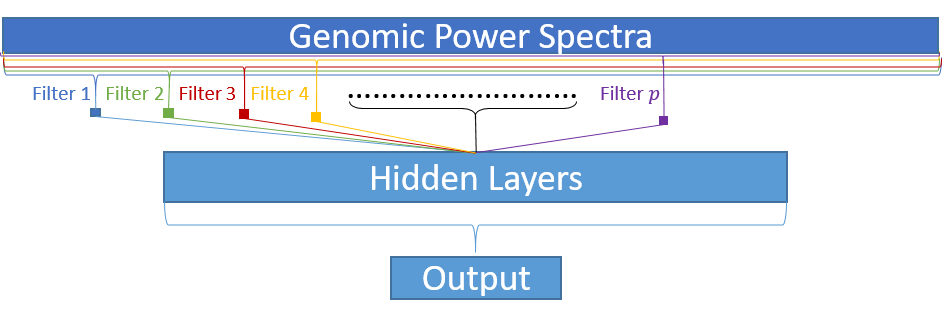
\includegraphics[scale=0.55]{Images/Files/afl.png}
\end{figure}

As with the previous approach, the size of the filtered PS can be selected by the researcher.
In this case, in contrast to the previous case, the resultant set of filtered PS coefficients actually consist of 
linear combinations of the unfiltered PS coefficients.  
In addition, this procedure is dependent on having supervised labels for the sequences used to construct 
the filters.  
These labels will determine the kinds of filters constructed and the information which they choose to 
emphasize, hence aspects of the original PS that help differentiate the elements of the 
sample on the chosen labels will be extracted by the filters learned.  

The convolutional network layer is applied to the entire length of the PS,  $p$, the number of filters to be learned by the 
CNN.  
The constructed filters also depend on the architecture of the hidden layers between the output 
and the convolutional layer.  
In the results section we will look at a specific architecture that learns filters by attempting to classify the 
region of submission sequences. 

\subsection{Maximal Variance Principal Components Filtering}

\noindent MVPCF provides filters in the same style as those automatically learned in AFL with the advantage of stronger correlation to distances calculated from the unfiltered PS.
For the largest subset of PS coefficients given $N$ samples, the principal components of the $N$ highest variance PS coefficients in the sample are taken as the filtered PS. 
When the number of samples, $N$, from which the filter is constructed is less than the length of the PS, $m$, 
this technique selects the $N$ highest variance PS coefficients, otherwise the entire PS is utilized. 
In this case, the selection of the length of the filtered PS is made by choosing only the first $k$ principal 
components. 

Let $\pmb{X}$ be the matrix containing PS of all samples from which we want to construct a filter, each row $i=1,2,\dots,N$ represents a signal, and each column $j=1,2\dots,m$ represents the $j$\textsuperscript{th} PS coefficient.  
A pre-filtering matrix $\pmb{H}$ may be determined from $\eta^*$ in Equation \ref{eq:var}, such that $\pmb{H}$ is of size $m \times k^*$, where $k^*$ is at most $N$. Each column of $\pmb{H}$ selects the single PS coefficient from $\pmb{X}$ of variance greater than $\eta^*$ and less than the previously selected PS coefficient, such that $\pmb{X}\pmb{H} = \pmb{X^*}$ is of size $N \times k^*$; thus, $\pmb{H}$ contains only contains only the maximal variance coefficients of $\pmb{X}$.  The singular value decomposition (SVD) of the matrix $\pmb{X^*}$ may be written $\pmb{X^*} = \pmb{U}\pmb{\Sigma}\pmb{W}^T$ with score matrix $\pmb{T} =\pmb{X^*}\pmb{W} = \pmb{U}\pmb{\Sigma}$. Then a post filtering matrix $\pmb{K}$ may 
be applied to the score matrix, such that $\pmb{K}$ is of size $k^* \times k$ and therefore $\pmb{T}\pmb{K} = \pmb{X^*}\pmb{W}\pmb{K} = \pmb{U}\pmb{\Sigma}\pmb{K} = \pmb{F}$ is the $N \times k$ \textit{maximal variance principal components filtered} representation of the initial PS matrix $\pmb{X}$. 

\section{Results} 
\label{sec:res}

\noindent In this section, the three filtering methods: MVF, AFL, and MVPCF are applied to a sample of viral genomes of the SARS-CoV-2 virus captured from the collection curated by the GISAID Initiative \cite{gisaid} on August 20, 2020.  Please see the acknowledgements for a link to the complete listing of labs contributing to GISAID.

\subsection{Minimal Variance Filtering} 
\vspace{-2 em} 

\begin{figure}[h!] 
\caption{(a) Scatter plot of PS coefficient variances for 1,397 SARS-CoV-2 Genomes, (b) Histogram of PS coefficient variances, (c) Survival Plot of Coefficients by Variance, (d) Pearson's $\rho$ between filtered PS distances and full PS distances. \label{fig:coeffvar}} 
\vspace{0.5 em}
\centering
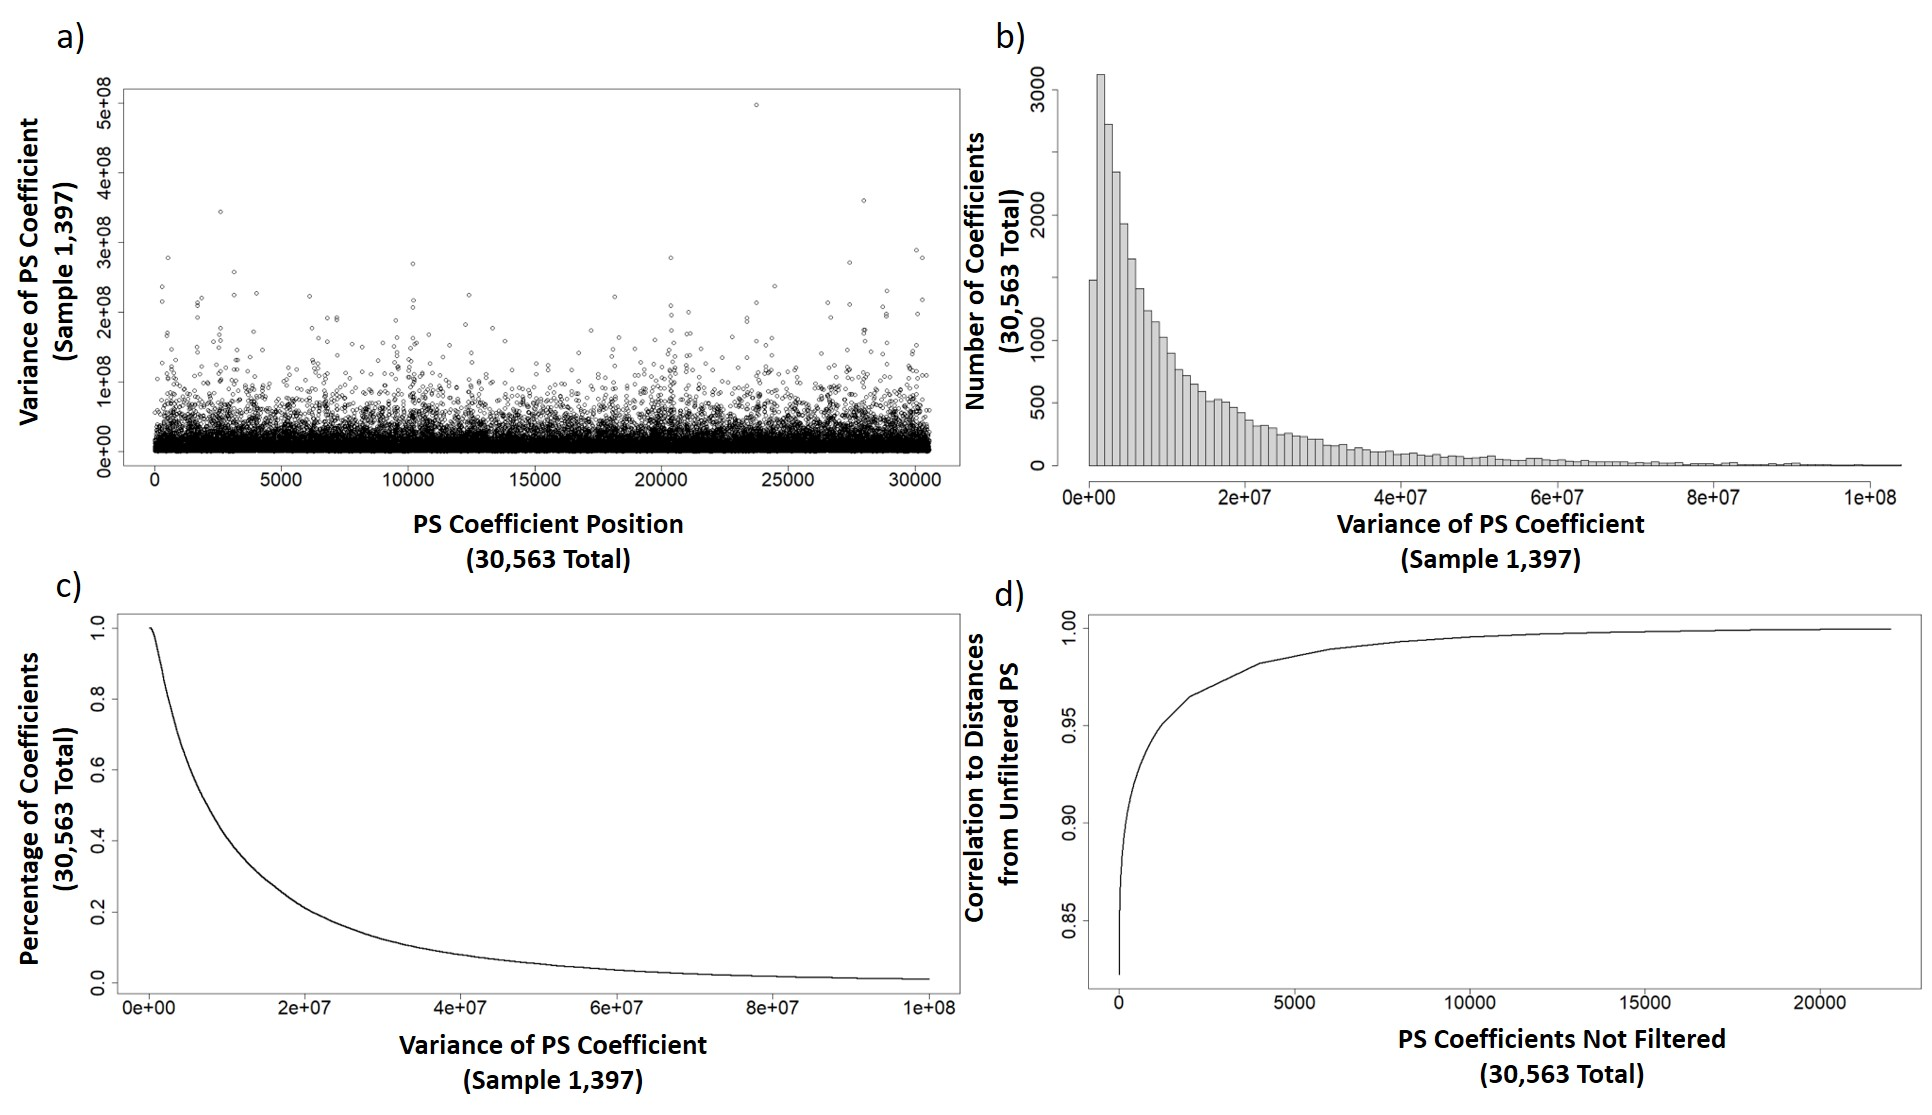
\includegraphics[scale=0.27]{Images/Files/VarianceFiltCombined.jpg}
\end{figure}

\noindent First, MVF is applied to the set of PS for the virus genomes. 
Figure \ref{fig:coeffvar} shows several views of the PS component variances for the data (the \textit{evenly-scaled} PS are of length 30,563), to assist with visualization of the Filter.
Figure \ref{fig:coeffvar} is intended to depict a few of the graphical displays of PS data that one may consider when designing a MVF and selecting the $\eta^*$ value. 


Figure \ref{fig:coeffvar} (a) is a scatter plot of the sample ($N=1,397$) variances PS Coefficient, $\eta^*$ may 
be graphically visualized as a horizontal line, below which PS coefficients are discarded. 
A histogram of PS coefficient variances in Figure \ref{fig:coeffvar} (b), allows graphical visualization of $\eta^*$ as a vertical line, left of which the area highlighted  provides the number of coefficients filtered.  
Figure \ref{fig:coeffvar} (c) is a survival curve of coefficients by their variance, that is, the
percentage of coefficients with variance greater than or equal to the ordinate is displayed as the 
abscissa. 
Figure \ref{fig:coeffvar} (d) displays the correlation of distances produced by the filtered and unfiltered PS for a range of coefficients filtered $q$. 


\subsection{Automated Filter Learning}


\begin{figure}[h!]
\centering
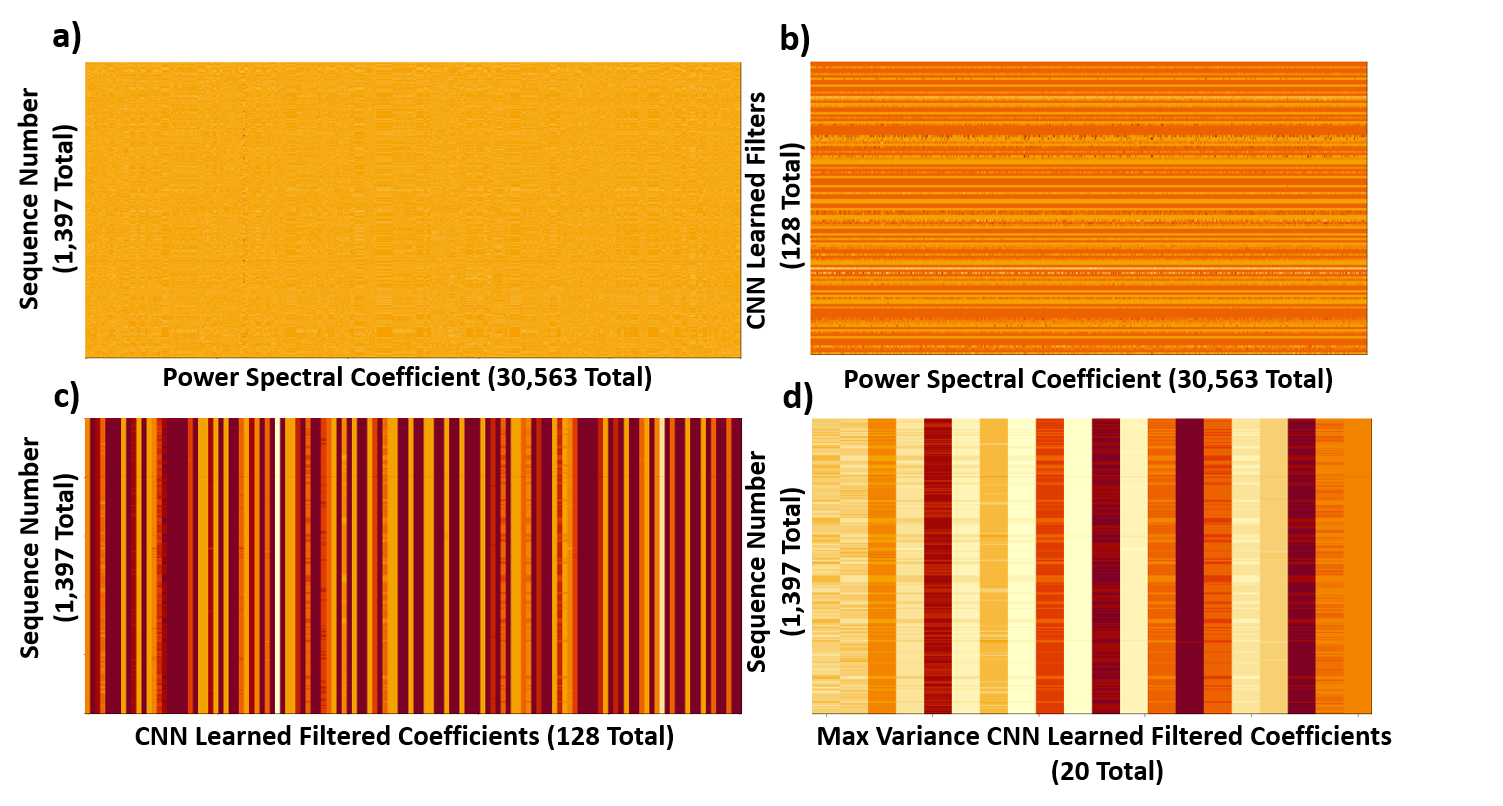
\includegraphics[scale=0.34]{Images/Files/CNNFilters.png}
\caption{(a) Image produced from scaled Unfiltered PS for all 1,397 Viral genomes (30,563 coefficients) (b) CNN Weights learned for 30,563 PS, for 128 Filters (c) Each of the 1,397 full PS (30,563) filtered into 128 values (d) The 20 highest variances filtered PS among the 128.  \label{fig:CNN128Filts}}
\end{figure}

A CNN for classifying the GISAID August SARS-CoV-2 PS by submission region for eight general regions extracted from the headers is implemented and trained using the \texttt{keras} package \cite{kerR21}.

The network used 128 filters spanning the full PS on all 1,397 sequences. 
It was trained for 20 epochs, using a batch size of 100.  
A graphical display of the learned filters is provided in Figure \ref{fig:CNN128Filts}.
For the comparison section, the CNN trains different numbers of filters to provide a 
valid filtered PS set for comparison to the other two methods. 
\subsection{Maximal Variance Principal Components Filtering}

\noindent In MVPCF there is an inherent 
restriction on the maximum size to which the sequence may be reduced.
Due to the nature of PCA, the number of components that can be produced from a set of sequences is limited by the number of sequences $N$.  
This $N$ is the maximum number of PS coefficients that may be considered when 
producing the filter, so in the case of these 1,397 viral genomes, we are limited to 
considerations of the PCA of the maximum variance 1,397 PS coefficients. 
As stated before, when $N$ is of greater length than $m$ this is not of concern, 
however in this case $N$ is 1,397, and $m$ is much larger than that (30,563). 
Of course, once the PCA of the 1,397 maximal variance coefficients is performed, 
selection of the first $k$ components allows for an even greater reduction.

\begin{figure}[h!] 
\centering
\caption{(a) Scree Plot showing Variance for first 10 principal components, (b) Biplot showing first component by second component \label{fig:PCAres}}
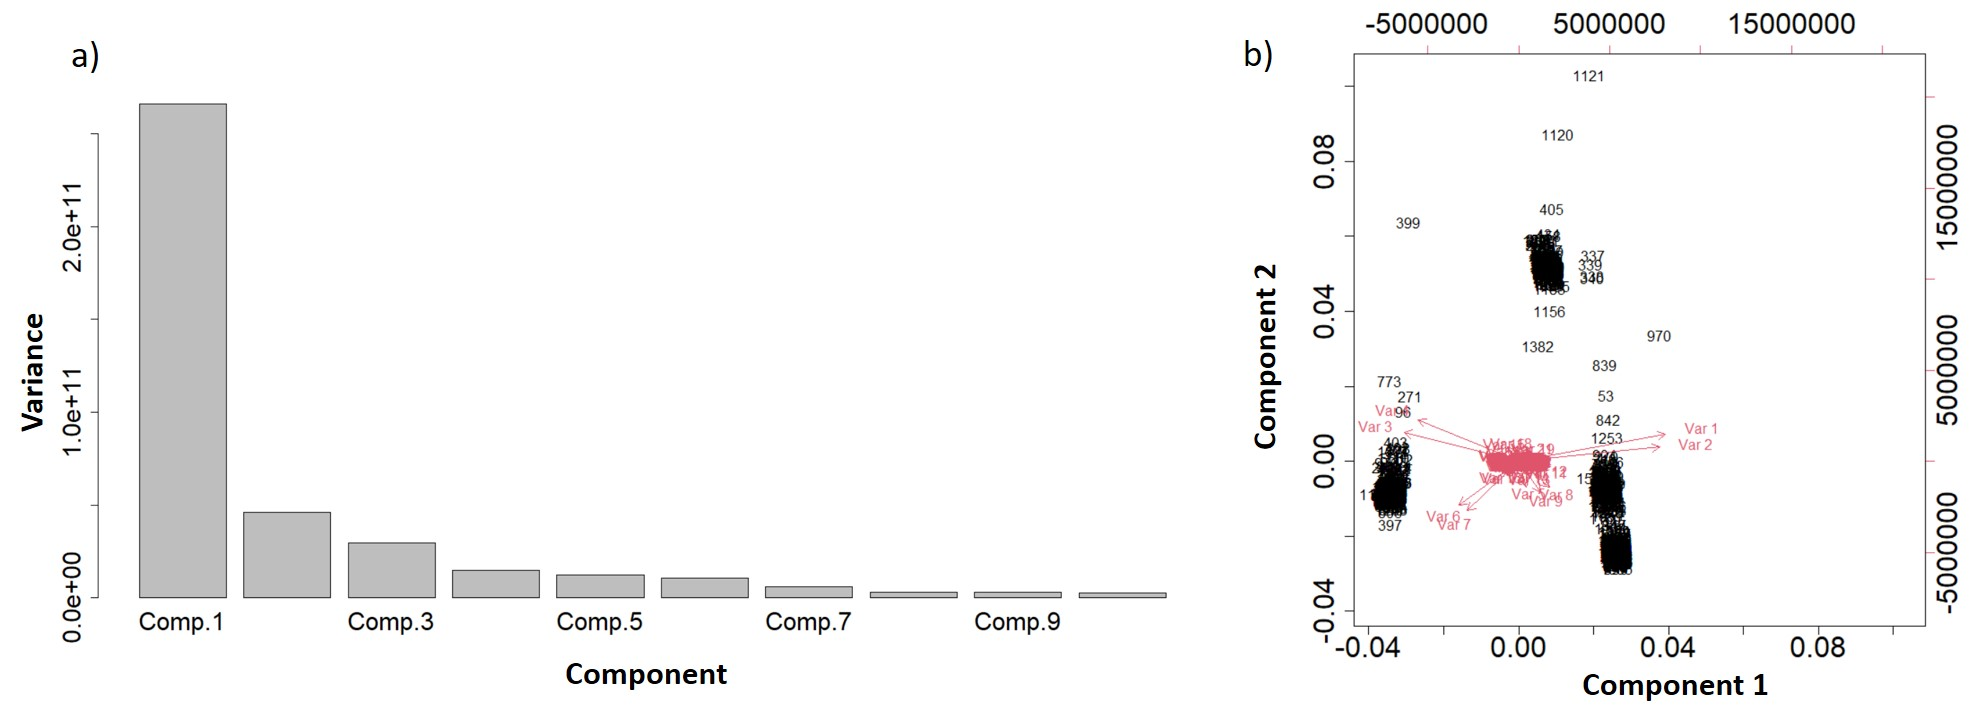
\includegraphics[scale=0.26]{Images/Files/PCAResults.jpg}
\end{figure} 

Figure \ref{fig:PCAres} provides visualization of the resulting PCA for the maximal
variance 1,397 elements of the PS.  The screeplot in Figure \ref{fig:PCAres} (a) 
shows that the vast majority of the variance of the set of maximal variance PS 
coefficients is contained in the first component, as we will see, distances calculated from this single value are correlated with distances calculated from the entire PS with $\rho \approx 0.88$.  The biplot in Figure \ref{fig:PCAres} (b) shows that even the first two coefficients provide a large seperation of the data, notably three pronounced clusters appear.
\vspace{-0.5 em}
\subsection{Method Comparison} 
\vspace{-0.5 em}
\begin{figure}[h!]
\centering
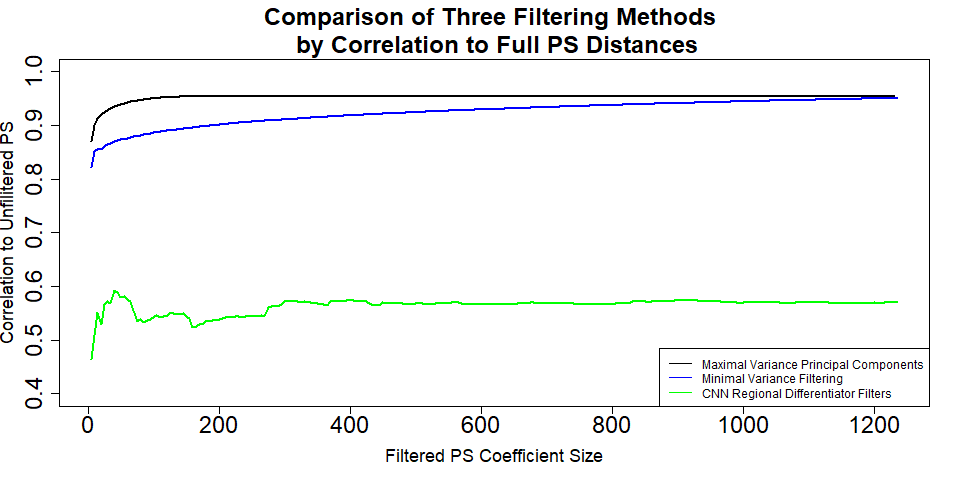
\includegraphics[scale=0.25]{Images/Files/PSFiltMethods.PNG}
\vspace{-0.5 em}
\caption{Filtering Methods Comparisons, by Correlation to Full PS Distances \label{fig:filtcomp}}
\end{figure}

\noindent MVPCF produces Euclidean distances which are most linearly related to the Euclidean distances computed from the full PS for the same number of coefficients in the other two methods, as per Figure \ref{fig:filtcomp}.
That said, recall that MVPCF has the ability to consider a maximum of only $N$ elements from the unfiltered PS (1,397 in this case).  Therefore, there must be some $N^* > N$ such that the MVF procedure will outperform the MVPCF's best possible correlation, which occurs at $N$. 
Perhaps one of the more surprising aspects of Figure \ref{fig:filtcomp} is the low correlation from the CNN trained filters.  
These filters extract information more relevant to differentiating the region of submission, than correlating to the full PS distances, and hence are not the best choice of the three methods for correlating to distances from the full PS.

\begin{table}[h!]
\centering
\caption{Random Forest of 500 trees CV Accuracies for Region Classification from Filtered PS ($\permil$)\label{tab:acc}} 
\begin{tabular}{|l | l | l | l|}
\hline 
\textbf{Filtered PS Size} & \textbf{MVF} & \textbf{AFL} & \textbf{MVPCF}\\ 
\hline 
\hline 
50 & 248.33 & \textbf{452.39} & 217.59\\ 
\hline
100 & 249.17 & \textbf{477.40} & 388.74 \\
\hline
250 & 310.03& 455.28 & \textbf{482.45} \\
\hline
500 & 287.06 & 482.44 & \textbf{485.32}\\
\hline
1000 & 454.51 & 445.16 & \textbf{485.32} \\
\hline
\end{tabular} 
\end{table}
 
 To compare filter efficiency at capturing potentially important information from the PS, five fold cross validation accuracy  of regional classification for the SARS-CoV-2 data with a random forest classifier (500 trees) [Africa (35), East Asia (257), Europe (678), Middle East (153), North America (42), Oceania (38), South America (89), West Asia (105)] are displayed in $\permil$ in table \ref{tab:acc}.  As we can see, the AFL method extracts the best information for discerning the region of submission lower sized filtered PS (as expected since these labels were used in training the filters), however for larger filter sizes, the MVPCF method actually produces a higher accuracy.  
 \vspace{-1 em}
\section{Conclusions}

\noindent Three non-parametric filter designs are described for genomic PS; MVF where PS coefficients with a between sample variance below a threshold $\eta^*$ determined by a supplied PS coefficient filtering percentage $q$ are discarded. In the SARS-CoV-2 case study, we show this approach to be straightforward, and allow for an excellent size reduction while distances computed using the filtered PS retain a high correlation to distances computed from the full unfiltered PS. AFL, where CNN's classifying sequences on extracted labels (region in the case study), did not provide filters producing distances which correlated as well with the unfiltered distances, suggesting that the filters produced in this procedure may not lend themselves well to representing the unfiltered PS, but perhaps better uses for these filters may be found in automated sorting procedures. MVPCF produces the best correlation for the largest PS size reductions in our case-study, and allows for excellent compression of the unfiltered PS. 

\label{sec:conc}

For future work, we will use pairwise ratios and differences the PS coefficients we will be able to use statistical hypothesis testing theory to derive expressions for the parameters of an asymptotic F and Variance-Gamma distribution respectively to create a test for whether two sequences come from the same source.  
A distributional test for the maximal PS coefficients based on the ratio/difference of the asymptotic distribution in the domain of attraction of the Gumbel distribution (as proven by McGee and Ensor \cite{mcg98}) could also be developed. 
As previously stated, these filtering techniques may be extended in a few directions, the automatic learning with the CNN can be extended to examine truly convolutional filters of shorter length than the full signal. 


\appendices
{\small
\section*{Acknowledgments}
\noindent The work in this paper would not have been possible without the support of the Daehwan Kim Lab in 
the Lyda Hill Department of Bioinformatics at UTSW.  In the results section the SARS-CoV-2 viral 
genomes captured from the GISAID Initiative \cite{gisaid} reflect the combined efforts of many labs, 
for a complete listing please see \url{https://tinyurl.com/8ptzru7s}.  \textbf{The authors would especially like to thank the organizers and reviewers of the BioCAS 2021 IEEE conference for their time, patience, and interest in the review of this work.}
\vspace{-1.5 em}
\begin{center}
\textsc{Thank You!}
\end{center}
\vspace{-1 em}

\bibliographystyle{IEEEtrans}

\bibliography{2021BioCASRef}
\vspace{-0.5 em}
\section{Acronym Dictionary} 
\vspace{-0.5 em}

\begin{itemize} 
\item \textbf{AFL} - Automated Filter Learning
\item \textbf{ASCII} - American Standard Code for Information Interchange
\item \textbf{BAM} - Binary Alignment Map. 
\item \textbf{CNN} - Convolutional Neural Network (Typically 1-Dimensional as applied to Genomic PS)
\item \textbf{CRAM} - Compressed Alignment Map.
\item \textbf{CV} - Cross Validation
\item \textbf{DFT} - Discrete Time Fourier Transform (Usually Discrete Loci, Mixed-Radix Transform)
\item \textbf{DNA} - Deoxyribonucleic Acids (Genetic Material stored in Eukaryotic Nuclei)
\item \textbf{FASTA/Q} - Fast-All File format (Q - Quality Scores)
\item \textbf{FFT} - Fast Fourier Transform (Usually Mixed Radix)
\item \textbf{GISAID} - Global Initiative on Sharing All Influenza Data (Initiative curating SARS-CoV-2 Genomes)
\item \textbf{IEEE} - Institute of Electrical and Electronics Engineers.
\item \textbf{ML} - Machine Learning
\item \textbf{MVF} - Minimal Variance Filtering
\item \textbf{MVPCF} - Maximal Variance Principal Component Filtering
\item \textbf{NT(s)} - Nucleotide(s) (referring arbitrarily to Adenine, Cytosine, Guanine, and Thymine (or Uracil))
\item \textbf{PCA} - Principal Components Analysis
\item \textbf{PS} - Power Spectra (Usually Mixed-Radix Fourier Power Spectra), Power Spectral  if followed by the word `coefficients'. 
\item \textbf{RNA} - Ribonucelic Acids (Genetic Material transcribed from DNA, existing outside Nuclei)
\item \textbf{SAM} - Sequence Alignment Map (A format usually outputted from aligners which displays the locations of reads along a reference). 
\item \textbf{SARS-CoV-2} - Sudden Acute Respiratory Syndrome Coronavirus 2 (Virus responsible for 2019- Pandemic)
\item \textbf{SMU} - Southern Methodist University (University in Dallas Texas) 
\item \textbf{SVD} - Singular Value Decomposition.
\item \textbf{UTSW} - University of Texas Southwestern (Medical Center \& University in Dallas, Texas)
\end{itemize}

\vspace{-0.5 em}
\section{Software Repository \& Tutorial Video}
\vspace{-0.5 em}

\noindent The R-Language was used for software development (R version 4.1.0 (2021-05-18) -- ``Camp Pontanezen") \cite{r21}.  The \texttt{keras} and \texttt{tensorFlow} R Interfaces are utilized \cite{kerR21,tfR21}.  The Genomic PS production is implemented in our R package \cite{dftR}, instructions for installation are on Github: \url{https://github.com/mathornton01/Genomic-DFT-Yin-R}. A short ($\approx$ 3:00) demonstrating the same, and discussing these filtering approaches is provided:\url{https://tinyurl.com/bxdw53z3}. The R-Code that produces the filters that are examined in this work is hosted on Github here: \url{https://tinyurl.com/Filtering-R-Code}.  
}

\pagebreak
\begin{IEEEbiographynophoto}{Micah Thornton}
Is a fourth year Ph.D. candidate in a joint Southern Methodist University (SMU) and University of Texas Southwestern (UTSW) Biostatistics Program.  Micah holds a Bachelor's of Science (B.S) in Computer Engineering, a B.S. in Statistical Science, and a Master's of Science (M.S) in Computer Engineering from SMU. 
\end{IEEEbiographynophoto}

\begin{IEEEbiographynophoto}{Monnie McGee} 
Is an associate professor in the Department of Statistical Science at SMU. Monnie holds a Bachelor's of Arts (B.A) in Mathematics and English from Austin College, and a Master's of Arts and Doctor of Philosophy in Statistics from Rice University.  

\end{IEEEbiographynophoto}

\end{document}


